% Cheyne Homberger - UMS talk 2012 - cheyne.homberger@gmail.com

\documentclass[xcolor=dvipsnames]{beamer}

% \usetheme[]{Hannover}
% \usetheme{Warsaw}
\usecolortheme[named=teal]{structure}
\setbeamerfont{frametitle}{size = {\Large}, family=\rmfamily}
\setbeamertemplate{navigation symbols}
% to make a handout, uncomment these
% \usepackage{pgfpages}
% \pgfpagesuselayout{8 on 1}

% packages for extra math symbols
\usepackage{amsthm, amsmath, amssymb} 

% I like these fonts better
\usepackage{palatino}
% \usepackage{palatino, mathpazo} 
% \renewcommand{\familydefault}{\rmdefault}

% lets you draw nice pictures
\usepackage{tikz}


\newcommand{\ds}{\displaystyle}
\newcommand{\ra}{\rightarrow}



% ===================================================================== %
\begin{document}
\title[Trees, Paths, Change]{\rmfamily \LARGE Trees, Paths, and Pocket Change\\
  \small An Introduction to Analytic Combinatorics}

\author{Cheyne Homberger}
\date{\today}

\begin{frame}
  \titlepage
\end{frame}

\section{Introduction}
\subsection{}


\begin{frame}{Plane Trees}
  \pause
  \begin{center}
    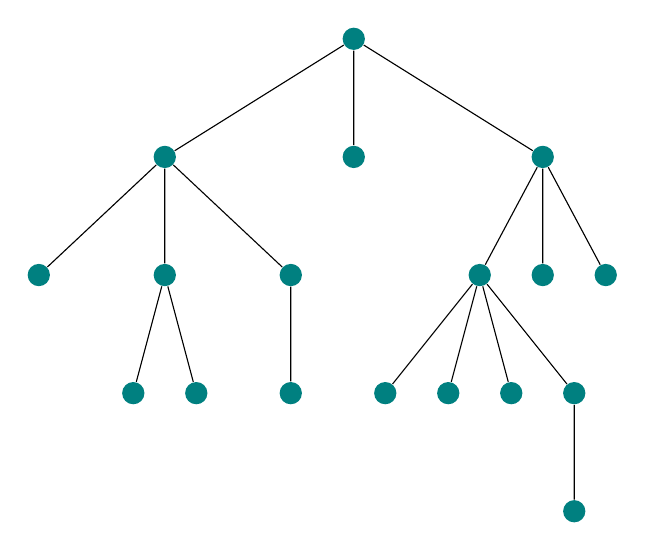
\begin{tikzpicture} % tikz is a nice scripting language for generating images
    % it can be hard to understand at first, but there are lots of examples and 
    % tutorials online (or you can use an open source program called geogebra,
    % which lets you see what you're drawing!)
    [level/.style={sibling distance=8mm},  
      dot/.style={circle, inner sep = 1mm,  fill = teal},
      scale = 1]
    \node[dot] at (0,0) {}
      child {node [dot] {}
        child {node [dot] {}}
        % empty child, to help with spacing
        child[fill = none] {edge from parent[draw=none]}
        child {node [dot] {} 
          child {node [dot] {}}
          child {node [dot] {}}
          }
        child[fill = none] {edge from parent[draw=none]}
        child {node [dot] {} 
          child {node [dot] {} }
          }
        }
      child[fill = none] {edge from parent[draw=none]}
      child[fill = none] {edge from parent[draw=none]}
      child {node [dot] {} }
      child[fill = none] {edge from parent[draw=none]}
      child[fill = none] {edge from parent[draw=none]}
      child {node [dot] {}
        child {node [dot] {}
          child {node [dot] {}}
          child {node [dot] {}}
          child {node [dot] {}}
          child {node [dot] {}
            child {node [dot] {}}
          }
        }
        child {node [dot] {}}
        child {node [dot] {}}};
    \end{tikzpicture}
  \end{center}
\end{frame}


\begin{frame}{Plane Trees}
  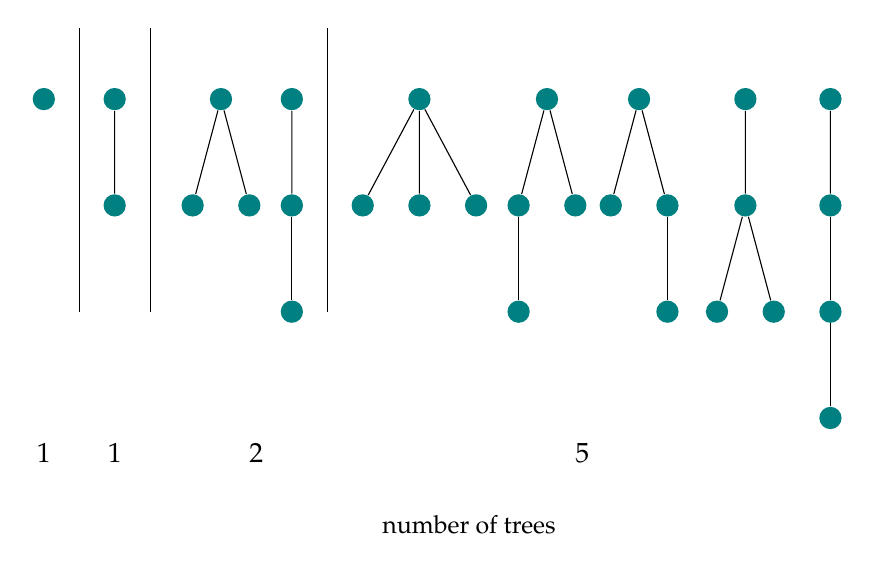
\begin{tikzpicture}
    [level/.style={sibling distance=8mm},  
      dot/.style={circle, inner sep = 1mm,  fill = teal},
      scale = .9, %grow'=up
      ]
     
    % \node at (6, 2) {\small number of nodes};
    \node at (6, -6) {\small number of trees};

    % \node at (0,1) {1};
    \node at (0,-5) {1};
    \node[dot] at (0,0) {};

    \pause
    
    \draw (.5, 1) -- (.5, -3);
    % \node at (1,1) {2};
    \node at (1,-5) {1};
    \node[dot] at (1,0) {}
      child {node [dot] {}};

    \pause
    
    \draw (1.5, 1) -- (1.5, -3);
    % \node at (3,1) {3};
    \node at (3,-5) {2};
    \node[dot] at (2.5,0) {}
      child {node [dot] {}}
      child {node [dot] {}};

    \node[dot] at (3.5,0) {}
      child {node [dot] {}
        child {node [dot] {}}
      };

    \pause

    \draw (4, 1) -- (4, -3);
    % \node at (7.6, 1) {4};
    \node at (7.6, -5) {5};
    \node[dot] at (5.3,0) {}
      child {node [dot] {}}
      child {node [dot] {}}
      child {node [dot] {}};

    \node[dot] at (7.1, 0) {}
      child {node [dot] {}
        child {node [dot] {} }}
      child {node [dot] {}};

    \node[dot] at (8.4, 0) {}
      child {node [dot] {}}
      child {node [dot] {}
        child {node [dot] {} }};

    \node[dot] at (9.9,0) {}
      child {node [dot] {} 
        child {node [dot] {} }
        child {node [dot] {}}};

    \node[dot] at (11.1, 0) {}
      child {node [dot] {}
        child {node [dot] {}
          child {node [dot] {}}}};
  \end{tikzpicture}
\end{frame}


\begin{frame}{Binary Trees}
  \pause
  \begin{center}
  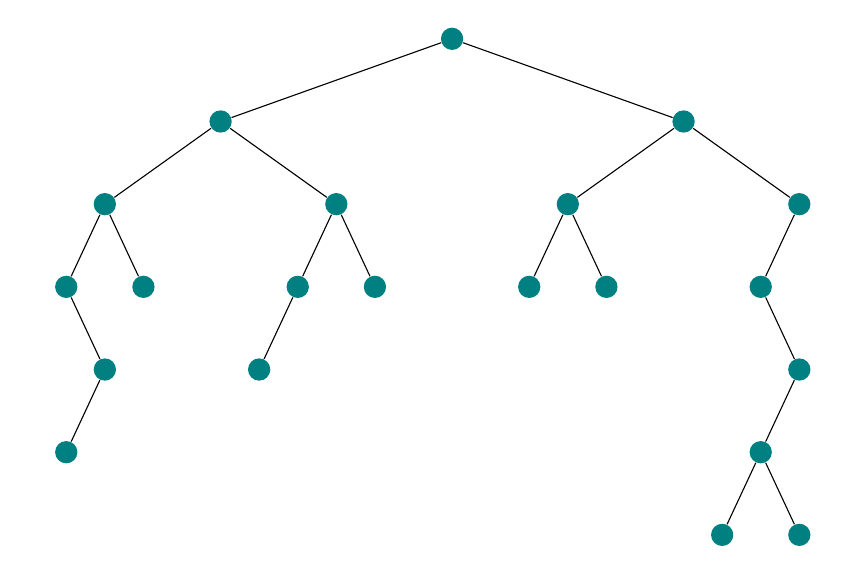
\begin{tikzpicture}
    [level/.style={sibling distance=14mm},  
      dot/.style={circle, inner sep = 1mm,  fill = teal},
      scale = .7]
    \node[dot] at (0,0) {}
      child {node [dot] {} 
        child {node [dot] {}
          child {node [dot] {}
            child[fill = none] {edge from parent[draw=none]}
            child {node [dot] {}
              child {node [dot] {}}
              child[fill = none] {edge from parent[draw=none]}
            }
          }
          child {node [dot] {}}
        }
      child[fill = none] {edge from parent[draw=none]}
      child[fill = none] {edge from parent[draw=none]}
      child {node [dot] {}
        child {node [dot] {}
          child {node [dot] {}}
          child[fill = none] {edge from parent[draw=none]}
          }
        child {node [dot] {}}
        }
      }
      child[fill = none] {edge from parent[draw=none]}
      child[fill = none] {edge from parent[draw=none]}
      child[fill = none] {edge from parent[draw=none]}
      child[fill = none] {edge from parent[draw=none]}
      child[fill = none] {edge from parent[draw=none]}
      child {node [dot] {} 
        child {node [dot] {}
          child {node [dot] {}}
          child {node [dot] {}}
        }
        child[fill = none] {edge from parent[draw=none]}
        child[fill = none] {edge from parent[draw=none]}
        child {node [dot] {}
          child {node [dot] {}
            child[fill = none] {edge from parent[draw=none]}
            child {node [dot] {}
              child {node [dot] {}
                child {node [dot] {}}
                child {node [dot] {}}
              }
              child[fill = none] {edge from parent[draw=none]}
            }
          }
        child[fill = none] {edge from parent[draw=none]}
        }
      };
  \end{tikzpicture}
  \end{center}
\end{frame}




\begin{frame}{Binary Trees}
  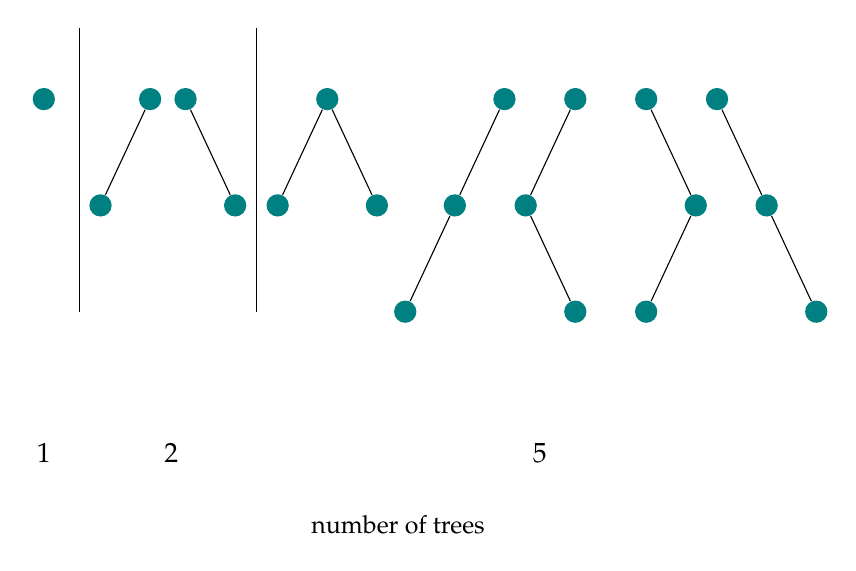
\begin{tikzpicture}
    [level/.style={sibling distance=14mm},  
      dot/.style={circle, inner sep = 1mm,  fill = teal},
      scale = .9]

    \node at (5, -6) {\small number of trees};

    % \node at (0,1) {1};
    \node at (0,-5) {1};
    \node[dot] at (0,0) {};

    \pause
    
    \draw (.5, 1) -- (.5, -3);
    % \node at (1,1) {2};
    \node at (1.8,-5) {2};
    \node[dot] at (1.5,0) {}
      child {node [dot] {}}
      child[fill = none] {edge from parent[draw=none]};

    \node[dot] at (2,0) {}
      child[fill = none] {edge from parent[draw=none]}
      child {node [dot] {}};

    \pause

    \draw (3, 1) -- (3, -3);
    \node at (7,-5) {5};
    \node[dot] at (4, 0) {}
      child {node [dot] {}}
      child {node [dot] {}};

    \node[dot] at (6.5,0) {}
      child {node [dot] {}
        child {node [dot] {}}
        child[fill = none] {edge from parent[draw=none]}}
      child[fill = none] {edge from parent[draw=none]};

    \node[dot] at (7.5,0) {}
      child {node [dot] {}
        child[fill = none] {edge from parent[draw=none]}
        child {node [dot] {}}}
      child[fill = none] {edge from parent[draw=none]};

    \node[dot] at (8.5,0) {}
      child[fill = none] {edge from parent[draw=none]}
      child {node [dot] {}
        child {node [dot] {}}
        child[fill = none] {edge from parent[draw=none]}};

    \node[dot] at (9.5,0) {}
      child[fill = none] {edge from parent[draw=none]}
      child {node [dot] {}
        child[fill = none] {edge from parent[draw=none]}
        child {node [dot] {}}};

  \end{tikzpicture}
\end{frame}


\begin{frame}{The Choose Function}
  \pause

  \begin{block}{Definition}
    $\displaystyle \binom{n}{k} = $ the number ways of picking $k$ objects from a collection
    of $n$ objects. \\
    \pause
    $\displaystyle \binom{n}{k} = \frac{n!}{k! (n-k)!} 
    = \frac{n(n-1)(n-2)\ldots (n - k + 1)}{k(k-1)(k-2) \ldots \cdot 3 \cdot 2 \cdot 1}$
  \end{block}
  \pause
  \begin{block}{Example}
  $\displaystyle \binom{5}{1} = 5$\\
  $\displaystyle \binom{5}{2} = \frac{5 \cdot 4}{2} = 10$
  \end{block}
\end{frame}


\begin{frame}{NS Paths}
  \pause
  \begin{center}
  \begin{tikzpicture}
    [dot/.style={circle, inner sep = 1mm,  fill = teal},
    scale = .8]
    \draw (0,0) -- (10,0);
    \pause
    \draw[->, >= latex] (0,0) -- (1,1);
    \pause
    \draw[->, >= latex] (1,1) -- (2,2);
    \pause
    \draw[->, >= latex] (2,2) -- (3,1);
    \pause
    \draw[->, >= latex] (3,1) -- (4,0);
    \pause
    \draw[->, >= latex] (4,0) -- (5,-1);
    \pause
    \draw[->, >= latex] (5,-1) -- (6,-2);
    \pause
    \draw[->, >= latex] (6,-2) -- (7,-1);
    \pause
    \draw[->, >= latex] (7,-1) -- (8,-2);
    \pause
    \draw[->, >= latex] (8,-2) -- (9,-1);
    \pause
    \draw[->, >= latex] (9,-1) -- (10,0);
  \end{tikzpicture}

  \vspace{2pc}
  \uncover<13->{
  \begin{tikzpicture}
    [dot/.style={circle, inner sep = 1mm,  fill = teal},
    scale = .8]
    \draw (0,0) -- (10,0);
    \pause
    \draw[->, >= latex] (0,0) -- (1,1);
    \pause
    \draw[->, >= latex] (1,1) -- (2,2);
    \pause
    \draw[->, >= latex] (2,2) -- (3,3);
    \pause
    \draw[->, >= latex] (3,3) -- (4,2);
    \pause
    \draw[->, >= latex] (4,2) -- (5,1);
    \pause
    \draw[->, >= latex] (5,1) -- (6,2);
    \pause
    \draw[->, >= latex] (6,2) -- (7,1);
    \pause
    \draw[->, >= latex] (7,1) -- (8,2);
    \pause
    \draw[->, >= latex] (8,2) -- (9,1);
    \pause
    \draw[->, >= latex] (9,1) -- (10,0);
  \end{tikzpicture}
  }

  \end{center}
\end{frame}


\begin{frame}{Dyck Paths}
  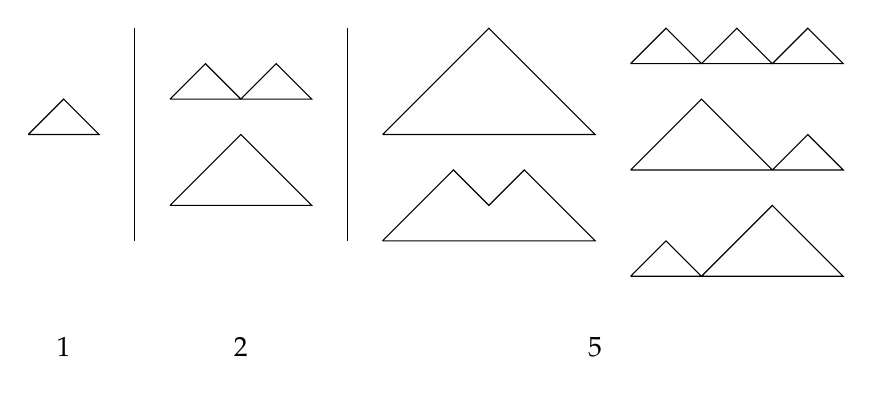
\begin{tikzpicture}
    [dot/.style={circle, inner sep = 1mm,  fill = teal},
    scale = .45]

    \node at (1, -6) {1};
    \draw (0,0) -- (2,0) -- (1,1) -- (0,0);

    \pause
    \draw (3,3) -- (3,-3);
    \node at (6, -6) {2};
    \draw (4, 1) -- (8,1) -- (7, 2) -- (6,1) -- (5,2) -- (4,1);
    \draw (4, -2) -- (8,-2) -- (7, -1) -- (6,0) -- (5,-1) -- (4,-2);

    \pause
    \draw (9,3) -- (9,-3);
    \node at (16, -6) {5};
    \draw (10, 0) -- (16, 0) -- (13,3) -- (10,0);
    \draw (10, -3) -- (16, -3) -- (14,-1) -- (13, -2) -- (12, -1) --(10, -3);
    \draw (17, 2) -- (23 , 2) -- (22,3)--(21,2)--(20,3)--(19,2)--(18,3)--(17,2);
    \draw (17,-1)--(19,1)--(21,-1)--(22,0)--(23,-1)--(17,-1);
    \draw (17,-4)--(18,-3)--(19,-4)--(21,-2)--(23,-4)--(17,-4);

  \end{tikzpicture}
\end{frame}


\begin{frame}{The Distributive Property}
  \pause
  \begin{block}{Fact} 
    $$c(a + b) = ca + cb$$
  \end{block}
\end{frame}


\begin{frame}
  \begin{block}{Binomial Theorem}
    $$(x + 1)^n = \sum_{k = 0}^n \binom{n}{k} x^k .$$
  \end{block}
  \pause

  \vspace{-2pc}

  \begin{proof}
    \small
    $$ \underbrace{(x+1)(x+1)(x+1) \ldots (x+1)}_\text{$n$ terms} =
      a_n x^n + a_{n-1}x^{n-1} + \ldots a_1 x + a_0 $$
      $$= \binom{n}{n}x^n + \binom{n}{n-1}x^{n-1} + \ldots \binom{n}{1}x + 
       \binom{n}{0} .  $$
  \end{proof}
  \pause

  \vspace{-1pc}

  \begin{block}{Corollaries}
    $$ 2^n = \sum_{k=0}^n \binom{n}{k} \pause \hspace{4pc} 0 = 
      \sum_{k=0}^n (-1)^k \binom{n}{k}.$$
  \end{block}
\end{frame}


\begin{frame}{Formal Power Series}
  \pause
  \begin{block}{Definition}
    $$ a_0 + a_1 x + a_2 x^2 + a_3 x^3 + \ldots = \sum_{n \geq 0} a_n x^n$$
    is called a \emph{power series}. If the $a_n$'s are zero after some point, we
    call it a polynomial.\\ \pause 
    This is \emph{not} a function, just an infinite sum of terms.
  \end{block}
  \pause
  $$ \Big(a_0 + a_1x + a_2 x^2 + \ldots\Big) +
    \Big(b_0 + b_1x + b_2 x^2 + \ldots \Big)$$
  $$ = (a_0 + b_0) + (a_1 + b_1)x + (a_2 + b_2)x^2 + \ldots $$
  \pause
  $$ \Big(a_0 +a_1x + a_2x^2 + \ldots \Big) 
    \Big(b_0 + b_1x +b_2x^2 +\ldots \Big)$$
  $$ \pause = a_0 b_0 + \pause(a_1b_0 + a_0b_1) x + 
    \pause (a_2b_0 + a_1b_1 + a_0b_2)x^2 + \ldots$$
\end{frame}


\begin{frame}
  \begin{block}{Example}
    $$ (1-x)(1 + x + x^2 + x^3 + \ldots ) = 1 + 0x + 0x^2 + \ldots$$
    \pause
    so 
    $$ \frac{1}{1-x} = 1 + x + x^2 + x^3 + \ldots .$$
  \end{block}
  \pause
  \begin{block}{Example}
    $$\frac{1}{(1-x)^2} = (1 + x + x^2 + \ldots )^2 = 
      \Big(1 + x + x^2 + \ldots \Big) \Big(1 + x + x^2 + \ldots \Big)$$
    \pause
    $$ = 1 \pause + (1 + 1)x \pause + (1+1+1)x^2 + \ldots $$
    \pause
    $$ = 1 + 2x + 3x^2 + 4x^3 + \ldots $$
  \end{block}
\end{frame}


\begin{frame}{Fibonacci Numbers}
  $$ f_0 = 1 \qquad f_1 = 1 \qquad f_n = f_{n-1} + f_{n-2} $$
  \pause
  $$ 1,1,\pause 2, \pause 3, \pause 5, \pause 8, \pause 13, 
    \pause 21,34, 55,89, \ldots $$
  \pause

  Let $\ds F = 1 + x + 2x^2 + 3x^3 + 5x^4 + 8x^5 + 13x^6 + \ldots $
  \vspace{1pc}

  \pause
  $$
  \begin{array}{rcccccc}
    xF =& & x+& x^2+ & 2x^3+& 3x^4 +& 5x^5 + 8x^6+ \ldots \\
    \pause
    +x^2F= & &  & x^2 +& x^3+& 2x^4 +& 3x^5 + 5x^6+ \ldots \\
    \hline \pause
    F = &1+ & x+& 2x^2+&3x^3+&5x^4 +& 8x^5 +13x^6 + \ldots
  \end{array} $$
  \pause
  $$ \begin{aligned} 
   &F = xF + x^2F + 1 \\ \pause
   &F - xF - x^2F = 1 \\ \pause
   &(1 - x - x^2) F = 1 \pause \rightarrow F = \frac{1}{1-x-x^2}
  \end{aligned} $$

\end{frame}


\begin{frame}{Fibonacci Numbers Cont'd}

  $$ \begin{aligned} 
    F &= \frac{1}{1 - x - x^2} \pause
      \hspace{2pc} 
     \alpha = \frac{-1+ \sqrt{5}}{2}, \beta=\frac{-1-\sqrt{5}}{2} \\ \pause
      &= \frac{-1}{(x-\alpha)(x-\beta)} \\ \pause
      &= \frac{A}{x - \alpha} + \frac{B}{x - \beta} \\ \pause
      &= \frac{-1/\sqrt{5}}{x - \alpha} - \frac{1/\sqrt{5}}{1-\beta} \\ \pause
      &= \frac{\alpha/\sqrt{5}}{1 - x/\alpha} - 
            \frac{\beta/\sqrt{5}}{1 - x/\beta} \\ \pause
      & \ldots \\
      & = \sum_{n \geq 0} \frac{\left(\frac{1+\sqrt{5}}{2}\right)^{n+1} - 
                \left(\frac{1 - \sqrt{5}}{2}\right)^{n+1}}{\sqrt{5}}x^n
        \pause  = f_0 + f_1 x + f_2 x^2 + \ldots
  \end{aligned}$$
\end{frame}


\begin{frame}{Making Change}
  \pause
  $$ Q = 1 + x^{25} + x^{50} + x^{75} + \ldots  = \frac{1}{1-x^{25}}$$
  \pause
  $$ D = 1 + x^{10} +x^{20} + x^{30} + \ldots = \frac{1}{1 - x^{10}}$$
  \pause
  $$ N = 1 + x^{5} +x^{10} + x^{15} + \ldots = \frac{1}{1 - x^{5}}$$
  \pause
  $$ P = 1 + x +x^{2} + x^{3} + \ldots = \frac{1}{1 - x}$$
  \pause
  What happens when we combine these?
\end{frame}


\begin{frame}{Making Change}
  $$QDNP = \frac{1}{(1-x)(1-x^5)(1-x^{10})(1-x^{25})}$$
  $$= (1 + x^{25}+\ldots)(1+x^{10}+\ldots)(1 + x^5 +\ldots)(1+x+\ldots)$$
  \pause
  $$ 1 + a_1x + a_2 x^2 + \ldots + a_{12}x^{12} + \ldots $$ \pause
  $$ = 1 + x + x^2 + x^3 + x^4 + 2x^5 + 2x^6 + 2x^7 + 2x^8 + 2x^9 $$
  $$ + 4x^{10} + 4x^{11} + 4x^{12} + 4x^{13} +4x^{14} + 
    6x^{15} + 6x^{16} + \ldots $$
  \pause
  What about no dimes? 
  $$QNP = 1 + x + x^2 + x^3 + x^4 + x^5 + 2x^6 + 2x^7 + 2x^8 + 2x^9$$
  $$+ 3x^{10} + 3x^{11} + 3x^{12} + 3x^{13} + 3x^{14} + 4x^{15} + 4x^{16} +
  \ldots $$ 
\end{frame}


\begin{frame}{Fixed Number of Coins}
  What if we also want to keep track of the total number of coins?
  \pause
  $$
  (1 + ux + u^2x^2 + \ldots ) \cdot
  (1 + ux^5 + u^2x^{10} + \ldots )$$
  $$ \cdot (1 + ux^{10} + u^2x^{20} + \ldots )\cdot
  (1 + ux^{25} + u^2x^{50} + \ldots )
  $$
  \pause
  $$ = \frac{1}{(1-ux)(1-ux^5)(1-ux^{10})(1-ux^{25})} = G(x,u)$$
  \pause
  $$ \begin{aligned}
  G(x,u) = \sum_{n,k \geq 0} a_{n,k}u^kx^n \pause &=
    \sum_{n\geq 0}x^n \left( \sum_{k \geq 0} a_{n,k} u^k\right) \\
    &= \sum_{k\geq 0}u^k \left( \sum_{n \geq 0} a_{n,k} x^n\right) 
    \end{aligned}
    $$
\end{frame}


\begin{frame}{Fixed Number of Coins}
  \begin{center}
  "I have two coins adding up to $35$ cents, and \emph{neither} coin is a dime"
  \pause
  \vspace{2pc}
  
  "No you don't"
  \end{center}
\end{frame}


\begin{frame}{Integer Partitions}
  \pause
  \begin{block}{Defintion}
    A \emph{partition} of an integer $n$ is a way of writing 
    $$ n = b_1 + b_2 + \ldots + b_k.$$
    \pause
    The number of ways of writing $n$ as a partition is denoted $p(n)$.  
  \end{block}
  \pause
  \begin{block}{Theorem}
    $$\begin{aligned} 
    \sum_{n \geq 0} p(n) x^n &= 
    (1 + x + \ldots)(1 + x^2 + \ldots) (1 + x^3 + \ldots) \ldots \\
      &= \frac{1}{(1-x)(1-x^2)(1-x^3) \ldots \ldots}
      \end{aligned}$$
    \pause
    $$  = 1 + x + 2x^2 + 3x^3 + 5x^4 + 7x^5 + 11x^6 + \ldots $$
  \end{block}
\end{frame}


\begin{frame}{Restricted Partitions}
  \pause
  \begin{block}{Definition}
    Let $p_d (n)$ be the number of partitions of $n$ into \emph{distinct}
    pieces. 
  \end{block}
  \begin{block}{Example}
    $p_d (5) = 3$, since 
    $$ 5 = 4 + 1 = 3 + 2 $$
  \end{block}
  \pause
  \begin{block}{Definition}
    Let $p_o(n)$ be the number of partitions of $n$ into \emph{odd} blocks.
  \end{block}
  \begin{block}{Example}
    $p_o(5) = 3$, since
    $$5 = 3 + 1 + 1 = 1 + 1 + 1 + 1$$
  \end{block}
\end{frame}


\begin{frame}{Restricted Partitions}
  \begin{block}{Theorem}
    $p_d(n) = p_o(n)$ for all positive integers $n$. 
  \end{block}
  \pause
  \begin{block}{Proof:} \small
    $$\begin{aligned}
    \sum_{n \geq 0} p_o x^n &= (1 + x + x^2 + \ldots)(1 + x^3 + x^6 + \ldots )
    \ldots \\
      \pause
      &= \frac{1}{(1-x)(1-x^3)(1-x^5) \ldots}\\
      \pause
      &= \frac{(1-x^2)(1-x^4)(1-x^6) \ldots}{(1-x)(1-x^2)(1-x^3)(1-x^4)(1-x^5)
      \ldots} \\
      \pause
      &= \left(\frac{1-x^2}{1-x}\right) 
          \left(\frac{1-x^4}{1-x^2}\right) 
          \left(\frac{1 - x^6}{1-x^3}\right) \ldots \\
      \pause
      &= (1+x) (1+x^2) (1+x^3) (1+x^4) (1+x^5) \ldots  \\
      \pause
      &= \sum_{n \geq 0} p_d(n) x^n 
      \pause
       \hspace{11pc} \qed \end{aligned} $$
  \end{block}
\end{frame}


\begin{frame}{Asymptotic Enumeration}
  \pause
  $$ a_n = \only<2>{\textcolor{black}{\sqrt{2} \cdot (4n+1)}}
          \only<3->{\textcolor{blue}{\sqrt{2} \cdot (4n+1)}}
       \only<2>{\textcolor{black}{\cdot 3^n}} 
       \only<3->{\textcolor{red}{\cdot 3^n}} $$

  \uncover<4>{
  $$ \textcolor{blue}{\sqrt{2} \cdot (4n+1)} \text{ is the \emph{subexponential}
  part}$$
  $$ \textcolor{red}{3^n} \text{ is the \emph{exponential} part} $$
  }
\end{frame}


\begin{frame}{Who cares about radius of convergence?}
  \pause
  $$ G(x) = \frac{1}{1-2x} = \sum_{n \geq 0} a_n x^n$$
  \pause

  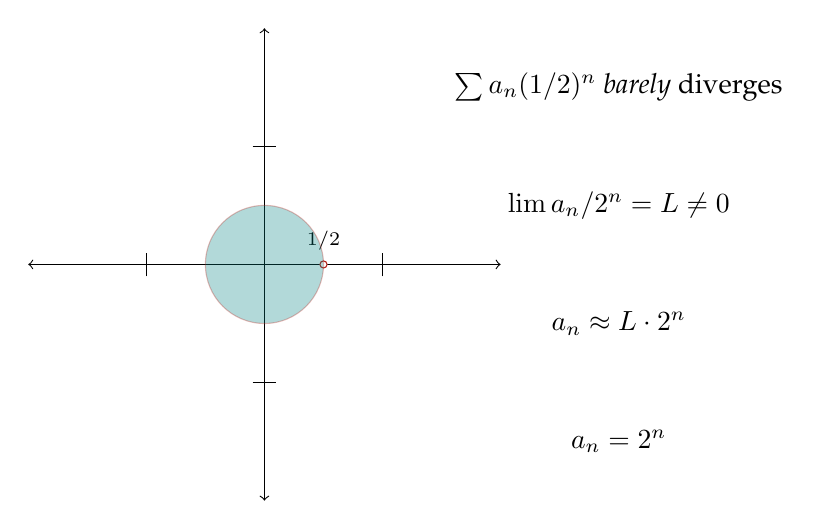
\begin{tikzpicture}
  [scale = 1.5] 
  \draw[<->] (-2,0) -- (2,0); 
  \draw[<->] (0,-2) -- (0,2); 
  \foreach \x in {-1, 1}
    \draw (\x, -.1) -- (\x, .1);
  \foreach \y in { -1, 1}
    \draw (-.1, \y) -- (.1, \y);
  \pause
  \draw[color = BrickRed, fill = white] (.5,0) circle (.3mm);
  \node at (.5,.2) {\scriptsize$1/2$};
  \pause
  \draw[color = BrickRed, fill = teal, opacity=.3] (0,0) circle (.5);
  \pause 
  \node at (3, 1.5) {$\sum a_n (1/2)^n$ \emph{barely} diverges};
  \node at (3, .5) {$\lim a_n/2^n = L \not = 0$};
  \pause
  \node at (3, -.5) {$ a_n \approx L \cdot 2^n$};
  \pause
  \node at (3, -1.5) {$ a_n = 2^n$};
  \end{tikzpicture}
\end{frame}


\begin{frame}{Fibonacci Asymptotics}
  \pause
  {  \small
    $$ \sum_{n\geq 0} f_n x^n = \frac{1}{1-x-x^2} =
    \frac{1}{(x-\alpha)(x-\beta)}, 
     \alpha = \frac{-1+ \sqrt{5}}{2} \beta=\frac{-1-\sqrt{5}}{2} $$
  }
  \pause
  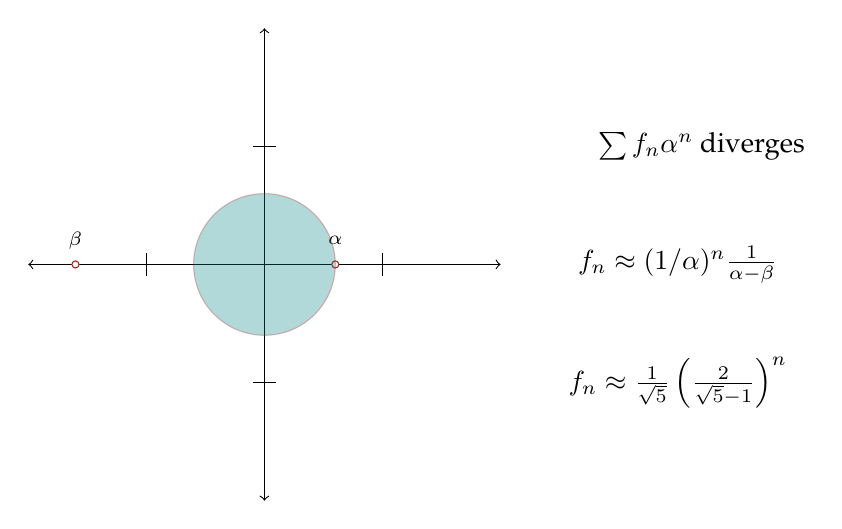
\begin{tikzpicture}
  [scale = 1.5] 
  \draw[<->] (-2,0) -- (2,0); 
  \draw[<->] (0,-2) -- (0,2); 
  \foreach \x in {-1, 1}
    \draw (\x, -.1) -- (\x, .1);
  \foreach \y in { -1, 1}
    \draw (-.1, \y) -- (.1, \y);
  \draw[color = BrickRed, fill = white] (.6,0) circle (.3mm);
  \node at (.6,.2) {\scriptsize$\alpha$};
  \draw[color = BrickRed, fill = white] (-1.6,0) circle (.3mm);
  \node at (-1.6,.2) {\scriptsize$\beta$};
  \pause
  \draw[color=BrickRed, fill=teal,  opacity=.3] (0,0) circle (.6);
  \pause
  \node at (3.7,1) {$ \sum f_n \alpha^n$ diverges};
  \pause
  \node at (3.5,0) {$f_n \approx (1/\alpha)^n \frac{1}{\alpha - \beta}$};
  \pause
  \node at (3.5,-1) {$f_n \approx \frac{1}{\sqrt{5}} 
      \left(\frac{2}{\sqrt{5} - 1}\right)^n$};

  \end{tikzpicture}
\end{frame}


\begin{frame}{Making change (asymptotically)}
  \small
  $$ \sum_{n \geq 0}c_n x^n = QDNP = \frac{1}{(1 - x^{25})(1-x^{10})(1-x^5)(1-x)} $$
  \pause
  $$  \frac{1}{(1-x)^4} \frac{1}{(1 + x + \ldots + x^{24})(1 + x + \ldots
      +x^9)(1 + x + \ldots + x^4)}$$
  \pause

  \vspace{1pc}

  $$ c_n \approx \frac{n^3}{3!} \cdot \frac{1}{25 \cdot 10 \cdot 5} = \frac{n^3}{7500}$$ 

  \pause 
  \vspace{1pc}

  Without dimes? 
  $$\frac{n^2}{250}$$
\end{frame}



\begin{frame}{Paths}
  \pause
  Let $p_n$ be the number of NS paths of length $2n$ that \emph{don't} cross
  below the $x$-axis, and let $ \ds P = \sum_{n \geq 0} p_n x^n$.
  \pause

  \vspace{1pc}

  \begin{tikzpicture}
  [scale = .6]
    \draw[color=white] (7,3)--(7,-5);
    \draw (0,0) -- (16,0);
    \draw[->, >= latex] (0,0) -- (1,1);
    
    \only<3-4>{
      \draw[->, >= latex] (1,1) -- (2,2);
      \draw[->, >= latex] (2,2) -- (3,1);
      \draw[->, >= latex] (3,1) -- (4,2);
      \draw[->, >= latex] (4,2) -- (5,3);
      \draw[->, >= latex] (5,3) -- (6,2);
      \draw[->, >= latex] (6,2) -- (7,1);
    }

    \only<5->{
      \node at (4, 2) {$P$};
      \node at (12, 1) {$P$};
      \draw (1,1) -- (7,1);
    }
    \only<4->{
      \draw (8,3) -- (8,-1);
    }

    \draw[->, >= latex] (7,1) -- (8,0);

    \only<3-4>{
      \draw[->, >= latex] (8,0) -- (9,1);
      \draw[->, >= latex] (9,1) -- (10,0);
      \draw[->, >= latex] (10,0) -- (11,1);
      \draw[->, >= latex] (11,1) -- (12,2);
      \draw[->, >= latex] (12,2) -- (13,1);
      \draw[->, >= latex] (13,1) -- (14,2);
      \draw[->, >= latex] (14,2) -- (15,1);
      \draw[->, >= latex] (15,1) -- (16,0);
    }
    \only<6->{
      \node at (3, -2) {$P = x \cdot P \cdot P + 1$};
    }
    \only<7->{
      \node at (9, -2) {$0 = xP^2 - P + 1$};
    }
    \only<8->{
      \node at (15, -2) {$ P = \frac{1 \pm \sqrt{1 - 4x}}{2x}$};
    }
    \only<9->{
      \node at (9, -4) {$\ds P = \frac{1 - \sqrt{1-4x}}{2x} = 
        1 + x + 2x^2 + 5x^3 + 14x^4 + \ldots $};
    }
  \end{tikzpicture}
\end{frame}


\begin{frame}{Binary Trees}
  Let $b_n$ be the number of binary trees with $n$ vertices, and let 
  $B = \sum_{n\geq 0} b_n x^n$. 

  \uncover<2->{
    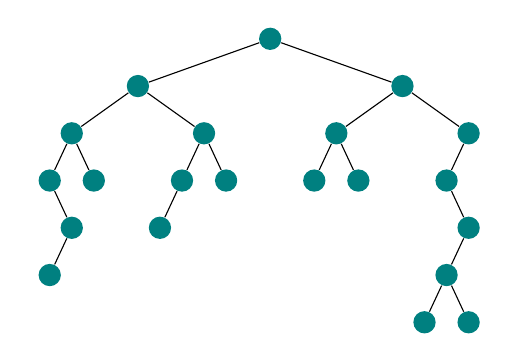
\begin{tikzpicture}
      [level/.style={sibling distance=14mm},  
        dot/.style={circle, inner sep = 1mm,  fill = teal},
        scale = .4]
      \node[dot] at (0,0) {}
        child {node [dot] {} 
          child {node [dot] {}
            child {node [dot] {}
              child[fill = none] {edge from parent[draw=none]}
              child {node [dot] {}
                child {node [dot] {}}
                child[fill = none] {edge from parent[draw=none]}
              }
            }
            child {node [dot] {}}
          }
        child[fill = none] {edge from parent[draw=none]}
        child[fill = none] {edge from parent[draw=none]}
        child {node [dot] {}
          child {node [dot] {}
            child {node [dot] {}}
            child[fill = none] {edge from parent[draw=none]}
            }
          child {node [dot] {}}
          }
        }
        child[fill = none] {edge from parent[draw=none]}
        child[fill = none] {edge from parent[draw=none]}
        child[fill = none] {edge from parent[draw=none]}
        child[fill = none] {edge from parent[draw=none]}
        child[fill = none] {edge from parent[draw=none]}
        child {node [dot] {} 
          child {node [dot] {}
            child {node [dot] {}}
            child {node [dot] {}}
          }
          child[fill = none] {edge from parent[draw=none]}
          child[fill = none] {edge from parent[draw=none]}
          child {node [dot] {}
            child {node [dot] {}
              child[fill = none] {edge from parent[draw=none]}
              child {node [dot] {}
                child {node [dot] {}
                  child {node [dot] {}}
                  child {node [dot] {}}
                }
                child[fill = none] {edge from parent[draw=none]}
              }
            }
          child[fill = none] {edge from parent[draw=none]}
          }
        };
    \end{tikzpicture}
  } 
  \only<3->{
    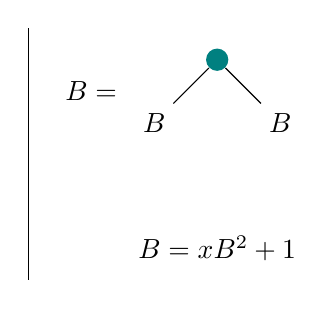
\begin{tikzpicture}
      [level/.style={sibling distance=14mm},  
        dot/.style={circle, inner sep = 1mm,  fill = teal},
        scale = .4]
      \node[dot] (root) at (0,0) {};
      \node (left) at (-2, -2) {$B$};
      \node (right) at (2, -2) {$B$};
      \draw (root) -- (left);
      \draw (root) -- (right);
      \node at (-4, -1) {$B = $};
      \node at (0, -6) {$B = xB^2 + 1$};
      \draw (-6,1) -- (-6, -7);
    \end{tikzpicture}
  }

  \vspace{1pc}

  \uncover<4>{
    $\ds P = \frac{1 - \sqrt{1-4x}}{2x} = 
      1 + x + 2x^2 + 5x^3 + 14x^4 + \ldots $
  }
\end{frame}



\begin{frame}{Plane Trees}
  \pause
  Let $t_n$ be the number of plane trees with $n$ vertices, and let 
  $T = \sum_{n \geq 0} t_n x^n $.

  \only<3->{
    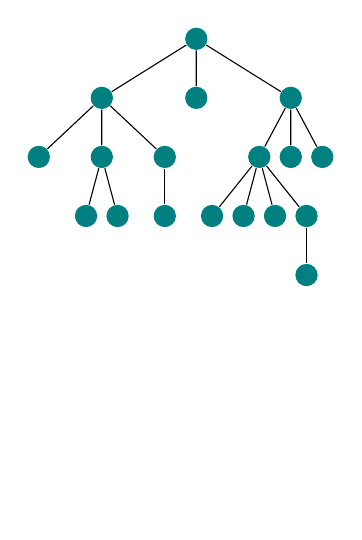
\begin{tikzpicture} 
      [level/.style={sibling distance=8mm},  
        dot/.style={circle, inner sep = 1mm,  fill = teal},
        scale = .5]
    \draw[color=white] (0,0) -- (0,-12);
      \node[dot] at (0,0) {}
        child {node [dot] {}
          child {node [dot] {}}
          % empty child, to help with spacing
          child[fill = none] {edge from parent[draw=none]}
          child {node [dot] {} 
            child {node [dot] {}}
            child {node [dot] {}}
            }
          child[fill = none] {edge from parent[draw=none]}
          child {node [dot] {} 
            child {node [dot] {} }
            }
          }
        child[fill = none] {edge from parent[draw=none]}
        child[fill = none] {edge from parent[draw=none]}
        child {node [dot] {} }
        child[fill = none] {edge from parent[draw=none]}
        child[fill = none] {edge from parent[draw=none]}
        child {node [dot] {}
          child {node [dot] {}
            child {node [dot] {}}
            child {node [dot] {}}
            child {node [dot] {}}
            child {node [dot] {}
              child {node [dot] {}}
            }
          }
          child {node [dot] {}}
          child {node [dot] {}}};
    \end{tikzpicture}
  }
  \pause
  \pause
    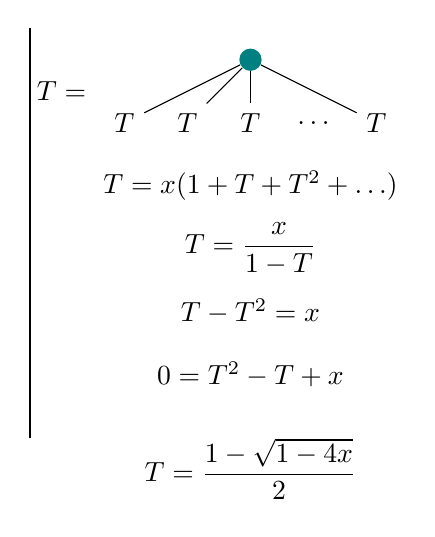
\begin{tikzpicture}
      [level/.style={sibling distance=14mm},  
        dot/.style={circle, inner sep = 1mm,  fill = teal},
        scale = .4]
      \node[dot] (root) at (0,0) {};
      \node (one) at (-4, -2) {$T$};
      \node (two) at (-2, -2) {$T$};
      \node (three) at (0, -2) {$T$};
      \node at (2, -2) {$\ldots$};
      \node (four) at (4, -2) {$T$};
      \draw (root) -- (one);
      \draw (root) -- (two);
      \draw (root) -- (three);
      \draw (root) -- (four);
      \node at (-6, -1) {$T = $};
      \draw (-7,1) -- (-7, -12);
      \pause
      \node at (0, -4) {$T = x(1 + T + T^2 + \ldots)$};
      \pause
      \node at (0, -6) {$\ds T = \frac{x}{1 - T}$};
      \pause
      \node at (0, -8) {$T - T^2 = x$};
      \pause
      \node at (0, -10) {$0 = T^2 - T + x$};
      \pause
      \node at (0, -13) {$\ds T = \frac{1 - \sqrt{1 - 4x}}{2}$};
    \end{tikzpicture}

\end{frame}



\begin{frame}{The Catalan Numbers}
  \pause
  $$ C = \frac{1 - \sqrt{1 - 4x}}{2x}$$
  \pause
  $$ C = \frac{1}{2x} - \frac{1}{2x} (1-4x)^{1/2} $$
  \pause
  $$ C = \frac{1}{2x} - \frac{1}{2x} \sum_{k \geq 0}\binom{1/2}{k} 4^n x^n $$
  \pause
  $$ \ldots $$
  $$ c_n = \binom{2n}{n} - \binom{2n}{n-1} = \frac{1}{n+1}\binom{2n}{n}$$
  \pause
  $$ 1, 1, 2, 5, 14, 42, 132, 429, 1430, \ldots $$
\end{frame}



\end{document}






